The problem tackled here is planning of (i) a dexterous grasp, (ii) for a novel object, (iii) given a single view of that object. The combination of constraints (i)-(iii) makes grasp planning hard because surface reconstruction will be partial, yet this cannot be compensated for by estimating pose for a known object model. This incompleteness in object surface reconstruction, together with additional uncertainty about object mass, co-efficients of friction, etcetera, renders infeasible the use of grasp planners which employ classical mechanics to predict grasp quality. Instead, we must employ a learning approach.

Grasp planning comprises two problems: generation and evaluation. Candidate grasps must be generated, and then each candidate must be evaluated, so as to produce a grasp quality measure (e.g maximum resistable wrench), the probability of grasp success, the likely in-hand slip or rotation, etcetera. These measures are then used to rank grasps so as to select one to execute.
\begin{figure}[t]
\begin{center}
  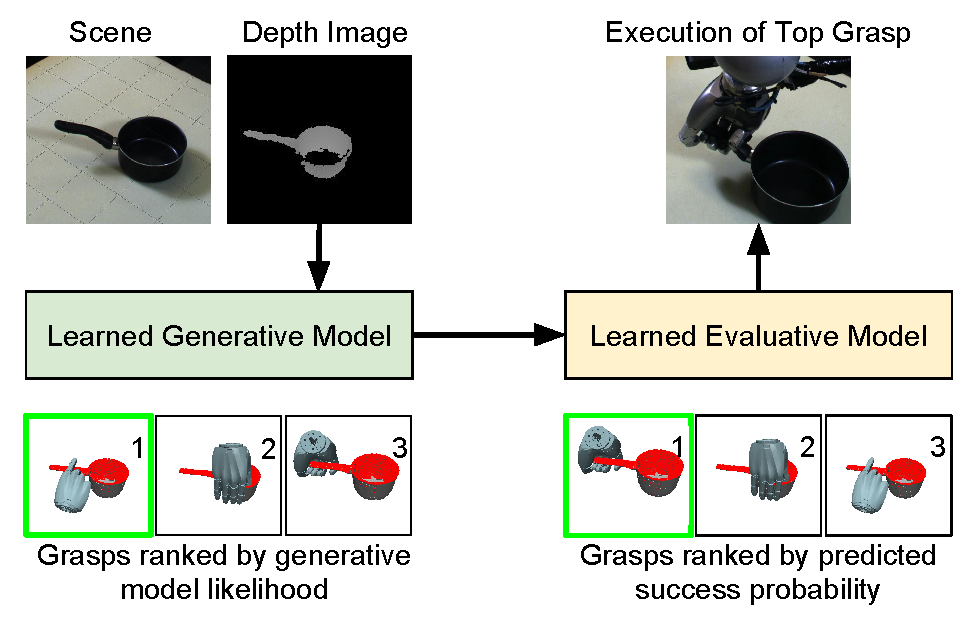
\includegraphics[width=0.9\columnwidth]{images/contribution.pdf}
  \end{center}
  \caption{The trained generative-evaluative system shown a novel object.}
\label{fig:systemArchitecture}
\end{figure}
Either or both a {\em generative} or {\em evaluative} model may be learned. If only a generative model is learned then evaluation must be carried out using mechanically informed reasoning, which cannot easily apply to our case of partial object reconstruction. If only an evaluative model is learned then grasp generation must proceed by search. This is challenging for dexterous grasping with up to 15 DoF. Thus, for dexterous grasping of novel objects from a single view, it becomes appealing to {\em learn} both the generative and the evaluative model. 

The contribution is the first generative-evaluative architecture where both generative and evaluative models are learned. A generative grasp model is learned from a small number of demonstrated grasps (10) using the data-efficient method for LfD. 
A data set is acquired by simulation of  grasps proposed by the generative model on novel objects. We vary parameters (mass, friction) which the robot cannot observe. This data set is used to learn an evaluative model using a deep net. This evaluative model is then used to rank grasps produced by the generative model for presentations of real novel objects. Unlike other approaches to deep grasping, which are restricted to power-grasps, the method is able to perform a wide variety of grasps, including pinch, rim, power, and handle grasps, and to use additional fingers to provide bracing.

The paper is structured as follows. First, we discuss related work. Second, the generative model is described. Third, we describe the architecture of the evaluative model. Fourth, we describe the design of the grasp simulation and the training of the evaluative model. Fifth, we present the experimental study.

